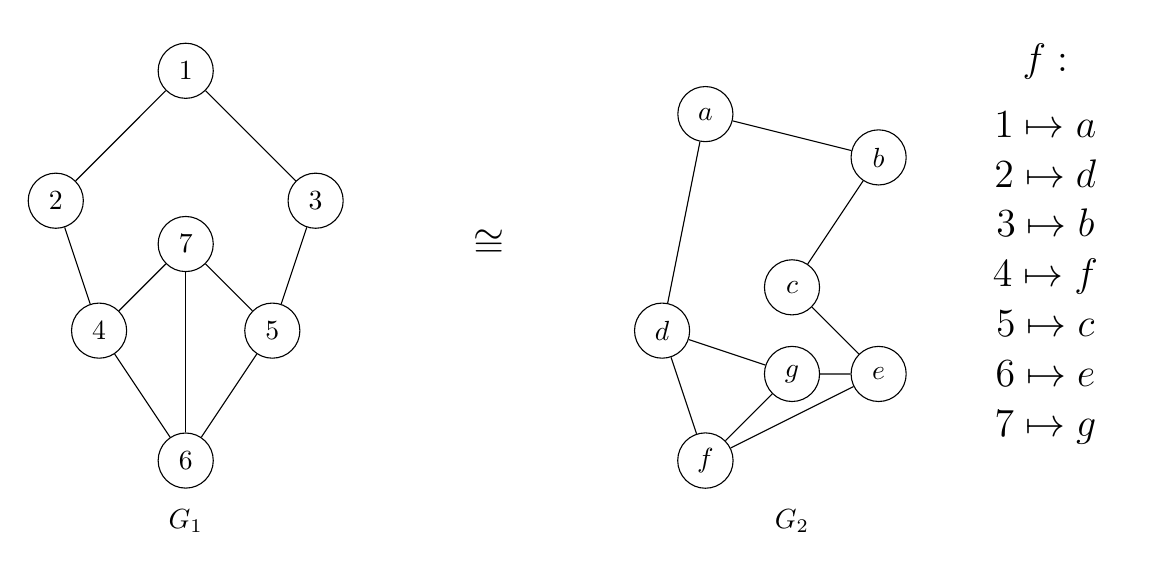
\begin{tikzpicture}[
    scale=1.1,
    every node/.style={circle, draw, minimum size=7mm}
]

% ================= G1 =================

\node (v1) at (0,2.5) {$1$};
\node (v2) at (-1.5,1) {$2$};
\node (v3) at (1.5,1) {$3$};
\node (v4) at (-1,-0.5) {$4$};
\node (v5) at (1,-0.5) {$5$};
\node (v6) at (0,-2) {$6$};
\node (v7) at (0,0.5) {$7$};

\draw (v1)--(v2);
\draw (v1)--(v3);
\draw (v2)--(v4);
\draw (v3)--(v5);
\draw (v4)--(v6);
\draw (v5)--(v6);
\draw (v4)--(v7);
\draw (v5)--(v7);
\draw (v6)--(v7);

\node[draw=none, rectangle] at (0,-2.7) {$G_1$};



% ================= G2 =================

\node (u1) at (6,2) {$a$};
\node (u2) at (8,1.5) {$b$};
\node (u3) at (7,0) {$c$};
\node (u4) at (5.5,-0.5) {$d$};
\node (u5) at (8,-1) {$e$};
\node (u6) at (6,-2) {$f$};
\node (u7) at (7,-1) {$g$};

\draw (u1)--(u2);
\draw (u1)--(u4);
\draw (u2)--(u3);
\draw (u3)--(u5);
\draw (u4)--(u6);
\draw (u5)--(u6);
\draw (u4)--(u7);
\draw (u5)--(u7);
\draw (u6)--(u7);

\node[draw=none, rectangle] at (7,-2.7) {$G_2$};



% ================= Isomorphism mapping =================

\node[
    draw=none,
    rectangle,
    align=left
] at (10,0.5)
{
\Large
\begin{tabular}{c}
$f:$\\[2mm]
$1 \mapsto a$\\
$2 \mapsto d$\\
$3 \mapsto b$\\
$4 \mapsto f$\\
$5 \mapsto c$\\
$6 \mapsto e$\\
$7 \mapsto g$
\end{tabular}
};


% Isomorphism symbol

\node[draw=none, rectangle] at (3.5,0.5)
{\Large $\cong$};

\end{tikzpicture}